\documentclass{article}
\usepackage{arxiv}
\usepackage[utf8]{inputenc}
\usepackage[T1]{fontenc}
\usepackage{hyperref}
\usepackage{url}
\usepackage{booktabs}
\usepackage{amsfonts}
\usepackage{amsmath}
\usepackage{amssymb}
\usepackage{nicefrac}
\usepackage{graphicx}
\usepackage{natbib}
\usepackage{doi}
\usepackage{tikz}
\usepackage{pgfplots}
\pgfplotsset{compat=1.18}
\usetikzlibrary{shapes,arrows,positioning,calc,backgrounds,fit,patterns,decorations.pathreplacing}
\usepackage{amsthm}
\usepackage{float}
\usepackage{algorithm}
\usepackage{algorithmic}

\newtheorem{proposition}{Proposition}
\newtheorem{hypothesis}{Hypothesis}
\newtheorem{definition}{Definition}

\title{Spatially-Informed Graph Variational Autoencoders Reveal Rare Immunosuppressive Tumor Microenvironment Subpopulations Predictive of Immunotherapy Resistance}

\author{
    Kundana Kommini$^{1}$, Maximilian Rutkowski$^{1}$, Brandon Yee$^{1}$\\
    $^{1}$Biology Lab, Yee Collins Research Group\\
    \texttt{\{k.kommini, m.rutkowski, b.yee\}@ycrg-labs.org}
}

\date{February 12, 2026}

\raggedbottom
\renewcommand{\headeright}{Preprint}
\renewcommand{\undertitle}{Preprint}
\renewcommand{\shorttitle}{Graph VAE for TME Analysis}

\begin{document}
\maketitle

\begin{abstract}
The tumor microenvironment (TME) orchestrates cancer progression and therapeutic resistance through complex cellular interactions that are poorly captured by conventional analysis methods. Here we propose a graph variational autoencoder (GVAE) framework that integrates single-cell RNA sequencing with spatial transcriptomics to model the TME as a relational network, enabling discovery of rare cell states and prediction of immunotherapy response. Our approach constructs cellular graphs where nodes represent individual cells with high-dimensional transcriptomic features, and edges encode both molecular similarity and spatial adjacency through a learned cell-adaptive gate that determines the per-cell balance between modalities. The GVAE encoder employs edge-weight-aware graph attention networks and reconstructs both graph topology via negative sampling and gene expression via a zero-inflated negative binomial decoder. A contrastive learning objective exploits spatial structure to learn embeddings where molecularly similar but spatially distant cells are distinguished. Rare immunosuppressive subpopulations are identified through KL divergence-based anomaly detection from the variational posterior, and their biological identity is confirmed through immunosuppressive gene signature scoring and pathway enrichment analysis. An end-to-end attention-pooling predictor enables patient-level response classification directly from cell embeddings. We validate this framework across four cancer types -- melanoma, lung, breast, and colorectal -- using publicly available datasets comprising over 300,000 cells with clinical response annotations. Head-to-head benchmarking against scVI and standard Scanpy workflows demonstrates the advantage of graph-based multi-modal integration, and cross-dataset transfer experiments from melanoma to NSCLC confirm generalizability of the learned representations. Systematic ablation studies across 12 conditions confirm the contribution of each architectural component. This work delivers a generalizable computational framework for multi-modal TME analysis, identification of rare but clinically relevant immunosuppressive cell states, and predictive biomarkers for immunotherapy response, released as open-source software.
\end{abstract}

\keywords{tumor microenvironment $\cdot$ graph neural networks $\cdot$ single-cell transcriptomics $\cdot$ spatial transcriptomics $\cdot$ immunotherapy $\cdot$ deep learning $\cdot$ variational autoencoders}

\section{Introduction}

\subsection{Clinical Motivation and Unmet Need}

Immunotherapy has fundamentally transformed cancer treatment over the past decade, offering durable responses and improved survival for patients with previously untreatable malignancies \citep{sharma2015future}. However, despite this revolutionary impact, clinical efficacy remains frustratingly limited, with only 20--40\% of patients responding to checkpoint blockade therapy across most cancer types \citep{haslam2019estimation}. This therapeutic ceiling represents not merely an incremental challenge but a fundamental barrier to realizing the full potential of immunotherapy. The primary determinant of therapeutic response lies within the tumor microenvironment (TME), a complex ecosystem comprising malignant cells, immune infiltrates, stromal components, and vascular elements that collectively orchestrate cancer progression and treatment resistance \citep{hinshaw2019tumor}.

The TME harbors immunosuppressive cell populations that actively mediate resistance to checkpoint inhibitors through diverse mechanisms including T cell exclusion, metabolic competition, and secretion of inhibitory cytokines \citep{cassetta2018targeting}. These immunosuppressive populations often comprise less than 5\% of total TME cells yet exert disproportionate influence on clinical outcomes \citep{murray2014macrophage}. Current computational approaches inadequately capture these rare but critical cell states, limiting our ability to predict therapy response and identify novel therapeutic targets. The challenge is further compounded by the spatial organization of the TME, where cellular neighborhoods and interaction networks fundamentally shape immune function \citep{binnewies2018understanding}. A macrophage proximal to the tumor-immune interface exhibits markedly different phenotypic and functional properties compared to an otherwise transcriptionally similar macrophage located in distal stroma, yet conventional single-cell analysis treats these cells as equivalent.

\subsection{Limitations of Current Analytical Approaches}

Despite remarkable technological advances in single-cell profiling technologies, computational methods for TME analysis have not kept pace \citep{stuart2019integrative}. Current approaches fall into three broad categories, each with fundamental limitations that constrain biological discovery and clinical translation.

First, conventional clustering methods such as those implemented in Seurat \citep{hao2021integrated} and Scanpy \citep{wolf2018scanpy} treat cells as independent observations, applying dimensionality reduction and clustering algorithms that implicitly assume statistical independence. This approach systematically discards information about cell-cell relationships, spatial organization, and interaction networks that are known drivers of TME function and immunosuppression \citep{palla2022squidpy}. Furthermore, standard clustering algorithms exhibit inherent bias toward abundant cell populations due to their reliance on distance metrics and density-based segmentation. Rare cell states comprising less than 5\% of the population are frequently absorbed into nearby abundant clusters or relegated to an undifferentiated ``other'' category, despite potentially harboring critical biological and clinical significance.

Second, ligand-receptor interaction analysis tools such as CellChat \citep{jin2021inference} and CellPhoneDB \citep{efremova2020cellphonedb} attempt to infer cellular communication by identifying co-expression of known ligand-receptor pairs across cell populations. While conceptually appealing, these methods suffer from several critical weaknesses. They generate thousands of predicted interactions without spatial validation, making it unclear which predictions represent genuine functional relationships versus statistical artifacts. The reliance on curated databases of known interactions limits discovery of novel communication mechanisms. Most fundamentally, these approaches perform inference post-hoc after cell type assignment, rather than integrating interaction information into the fundamental process of cell state definition.

Third, spatial analysis frameworks such as Squidpy \citep{palla2022squidpy} and Giotto \citep{dries2021giotto} provide sophisticated tools for analyzing spatial patterns in tissue sections. However, these methods typically analyze spatial organization after clustering has been performed on molecular features alone. This sequential approach means that spatial information does not influence the fundamental definition of cell states, potentially missing transcriptionally similar but spatially distinct populations with divergent biological functions.

\subsection{Graph Neural Networks as a Transformative Framework}

Graph neural networks (GNNs) have emerged as a powerful paradigm for learning from relational data across diverse domains including social network analysis, molecular chemistry, and knowledge graphs \citep{wu2020comprehensive}. The fundamental insight underlying GNNs is that many real-world systems are naturally represented as graphs, where entities (nodes) are connected by relationships (edges), and both structural topology and node features jointly determine system behavior.

The TME is fundamentally a relational system where cellular phenotypes and functions emerge from networks of cell-cell interactions mediated by direct contact, paracrine signaling, and spatial proximity \citep{armingol2021deciphering}. Graph-based representations offer a natural and biologically motivated framework for TME analysis. Despite this conceptual alignment and the demonstrated success of GNNs in other biological applications \citep{zitnik2018modeling}, graph-based deep learning remains substantially underutilized in TME research.

\subsection{Variational Autoencoders for Uncertainty Quantification}

Variational autoencoders (VAEs) extend traditional autoencoders by learning a probabilistic latent representation rather than a deterministic embedding \citep{kingma2013auto}. This probabilistic formulation provides several critical advantages for biological data analysis. First, VAEs naturally quantify uncertainty through the learned variance of the latent distribution, enabling identification of cells with ambiguous or transitional states. Second, the variational inference framework provides a principled approach to handling the high levels of technical noise inherent in single-cell data. Third, the regularization imposed by the Kullback-Leibler divergence term encourages learning of disentangled, interpretable latent representations.

Graph variational autoencoders (GVAEs) \citep{kipf2016variational} combine the relational learning capacity of GNNs with the probabilistic framework of VAEs. The variational formulation is particularly valuable for rare cell detection, as the learned uncertainty estimates can identify unusual cells that deviate from the typical latent manifold. Despite these attractive properties, GVAEs have not been systematically developed or validated for integrated analysis of single-cell and spatial transcriptomics data.

\subsection{Research Objectives and Expected Impact}

This research introduces a novel GVAE framework specifically designed for integrated analysis of single-cell RNA sequencing and spatial transcriptomics to comprehensively characterize the TME. Our approach addresses the critical limitations of existing methods through five key innovations: (1) a cell-adaptive gate mechanism that learns the per-cell balance between molecular and spatial information; (2) a zero-inflated negative binomial expression decoder that reconstructs gene expression alongside graph topology; (3) a contrastive learning objective that exploits spatial structure to distinguish molecularly similar but spatially distant populations; (4) KL divergence-based rare cell detection from the variational posterior; and (5) an end-to-end attention-pooling predictor for patient-level immunotherapy response.

We validate this framework across four major cancer types using publicly available datasets comprising over 300,000 cells with clinical annotations, perform systematic ablation studies across 12 conditions, benchmark against established methods (scVI and standard Scanpy workflows), and demonstrate cross-dataset generalizability through transfer experiments.

\section{Related Work}

\subsection{Single-Cell Transcriptomics Analysis Methods}

The revolution in single-cell RNA sequencing technologies over the past decade has enabled unprecedented molecular profiling of individual cells within complex tissues \citep{tanay2017scaling}. Seurat \citep{satija2015spatial} emerged as one of the first comprehensive toolkits, introducing anchor-based integration methods for combining datasets across batches and experimental conditions. Scanpy \citep{wolf2018scanpy} provided a Python-based alternative with scalable implementations designed to handle datasets exceeding one million cells.

These clustering-based approaches have become the de facto standard for single-cell analysis, typically following a sequential pipeline of quality control, normalization, highly variable gene selection, dimensionality reduction via principal component analysis, construction of k-nearest neighbor graphs in PCA space, and community detection using algorithms such as Leiden \citep{traag2019louvain}. While computationally efficient and broadly applicable, these methods treat cells as independent observations and rely heavily on Euclidean distances in gene expression space. Recent benchmarking studies have revealed that clustering results can be highly sensitive to preprocessing choices, parameter settings, and algorithm selection \citep{luecken2019current}.

Deep learning approaches have increasingly been applied to overcome limitations of linear dimensionality reduction. scVI (single-cell Variational Inference) \citep{lopez2018deep} employs a VAE framework to learn a low-dimensional latent representation while explicitly modeling technical noise sources including library size variation and batch effects through a zero-inflated negative binomial observation model. SAUCIE \citep{amodio2019exploring} combines autoencoders with information theory-based regularization to learn interpretable representations. However, none of these methods explicitly model cell-cell relationships or integrate spatial information into their architecture.

\subsection{Spatial Transcriptomics Technologies and Analysis}

Spatial transcriptomics has emerged as a transformative complement to single-cell RNA sequencing, enabling measurement of gene expression while preserving the native tissue architecture \citep{moses2022museum}. Visium (10x Genomics) performs transcriptome-wide profiling of 55-micron diameter spots, with recent Visium HD technology reducing resolution to subcellular scale. Targeted spatial technologies such as Xenium and CosMx achieve single-cell resolution for predefined gene panels.

Analytical methods for spatial transcriptomics have evolved rapidly. Squidpy \citep{palla2022squidpy} provides a comprehensive framework for spatial analysis including neighborhood enrichment testing, spatial autocorrelation via Moran's I, and identification of spatially variable genes. Deconvolution methods such as Cell2Location \citep{kleshchevnikov2022cell2location} and RCTD \citep{cable2022robust} use single-cell RNA-seq reference atlases to infer cell type composition of spatial spots. However, existing spatial analysis methods typically operate on predefined cell type annotations derived from molecular data alone, rather than jointly learning cell states from integrated molecular and spatial features.

\subsection{Graph Neural Networks in Biological Applications}

Graph neural networks have demonstrated remarkable success in biological applications where relational structure is fundamental to system behavior \citep{zhou2020graph}. In molecular property prediction, GNNs learn representations of chemical compounds by iteratively aggregating information from bonded atoms \citep{gilmer2017neural}. In protein structure prediction, GNNs operate on residue contact graphs \citep{ingraham2019generative}. Applications of GNNs to single-cell transcriptomics data have been more limited but are rapidly emerging. scGNN \citep{wang2021scgnn} constructs a cell-cell similarity graph and applies graph convolutional networks for imputation and clustering. However, these applications treat the graph structure as a preprocessing step rather than as a fundamental representation for biological discovery. Critically, none of these methods integrate spatial information into the graph construction or leverage the graph structure for unsupervised discovery of spatially-restricted cell states.

\subsection{Cell-Cell Communication Inference}

CellPhoneDB \citep{efremova2020cellphonedb} pioneered computational inference of ligand-receptor interactions by testing for enriched co-expression of known receptor-ligand pairs across cell type clusters. CellChat \citep{jin2021inference} extends this framework by incorporating multi-subunit complexes, cofactors, and signaling pathway annotations. NicheNet \citep{browaeys2020nichenet} integrates gene regulatory network information to predict how ligands from sender cells influence target gene expression. These methods suffer from reliance on curated databases and perform inference without considering spatial relationships, leading to biologically implausible interaction predictions for cell types that never occupy the same spatial neighborhood.

\subsection{Deep Learning for Immunotherapy Response Prediction}

Prediction of immunotherapy response remains one of the most pressing challenges in precision oncology, with existing biomarkers such as PD-L1 expression and tumor mutational burden providing only modest predictive accuracy \citep{jardim2021role}. Analysis of TME cellular composition has revealed associations between immune infiltration patterns and therapeutic response. High densities of CD8+ T cells correlate with better outcomes \citep{tumeh2014pd}, while abundance of immunosuppressive cell types predicts resistance \citep{cassetta2018targeting}. However, cell type proportion-based models explain only a modest fraction of response variance, suggesting that more sophisticated representations of TME organization are needed. No existing work has integrated graph-based deep learning representations of the TME with end-to-end predictive modeling for immunotherapy response, representing a significant methodological gap with clear translational relevance.

\section{Methodology}

\subsection{Overview of Analytical Framework}

Our methodological approach integrates single-cell RNA sequencing and spatial transcriptomics data through a graph-based deep learning framework centered on variational autoencoders. The analytical pipeline proceeds through six major stages (Figure~\ref{fig:framework}): (1) data acquisition, quality control, and preprocessing; (2) construction of cellular graphs encoding molecular similarity and spatial adjacency with a learned cell-adaptive gate; (3) training of graph variational autoencoders with multi-component loss functions to learn low-dimensional latent representations; (4) two-phase training with representation learning followed by clinical fine-tuning; (5) downstream analysis including uncertainty-aware clustering, KL-based rare cell detection, immunosuppressive signature validation, and clinical association testing; and (6) benchmarking against baseline methods and cross-dataset transfer evaluation. This section details each component with sufficient specificity to enable independent reproduction.

\begin{figure}[t]
\centering
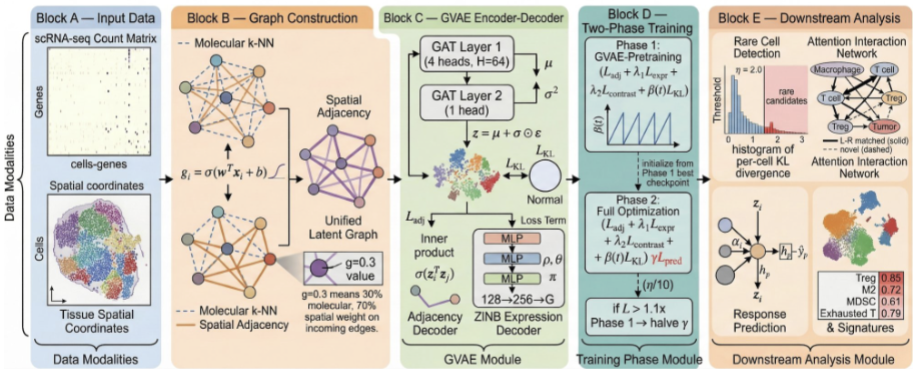
\includegraphics[width=\textwidth]{figuresGVAE/Framework.png}
\caption{\textbf{Overview of the GVAE framework for tumor microenvironment analysis.} The pipeline proceeds from input data modalities (scRNA-seq count matrices and spatial coordinates) through graph construction with a learned cell-adaptive gate, to the GVAE encoder-decoder architecture producing latent cell embeddings. A two-phase training protocol first learns biological representations, then fine-tunes for clinical prediction. Downstream modules perform rare cell detection via KL divergence thresholding, attention-based interaction network analysis, end-to-end immunotherapy response prediction via attention pooling, and uncertainty-aware clustering with immunosuppressive signature validation.}
\label{fig:framework}
\end{figure}

\subsection{Data Acquisition and Preprocessing}

\subsubsection{Dataset Selection and Characteristics}

We analyze publicly available single-cell and spatial transcriptomics datasets spanning four major cancer types: melanoma, non-small cell lung carcinoma (NSCLC), breast cancer, and colorectal cancer. Datasets were selected based on five criteria: presence of TME heterogeneity including tumor, immune, and stromal cell populations; adequate sample size; high data quality with median genes per cell exceeding 200; availability of clinical annotations including therapy response; and availability of matched or comparable spatial transcriptomics data. Table \ref{tab:datasets} summarizes the primary datasets.

\begin{table}[t]
\centering
\caption{Primary datasets for tumor microenvironment graph analysis}
\label{tab:datasets}
\begin{tabular}{llrrl}
\toprule
Cancer Type & Technology & Cells/Spots & Patients & Accession \\
\midrule
Melanoma & scRNA-seq (10x) & 16,291 & 32 & GSE120575 \\
Breast (ER+/HER2+) & scRNA-seq (10x v3) & 45,000 & 8 & GSE243280 \\
NSCLC & scRNA-seq (10x 5') & 9,000 & 1 & 10x Genomics$^\dagger$ \\
NSCLC & Visium HD (16$\mu$m bins) & 5,000 & 1 & 10x Genomics$^\dagger$ \\
NSCLC (ICI cohort) & scRNA-seq (10x) & 200,000+ & 243 & GSE243013 \\
Colorectal & Visium HD & 50,000 & 3 & GSE280318 \\
\bottomrule
\multicolumn{5}{l}{\footnotesize $^\dagger$Manufacturer demonstration datasets, used for spatial integration development only.}
\end{tabular}
\end{table}

The melanoma dataset \citep{sade2018defining} provides the primary cohort for immunotherapy response prediction, comprising 48 samples from 32 patients treated with anti-PD-1 checkpoint blockade with responder/non-responder annotations. The NSCLC ICI cohort \citep{deng2025nsclc} provides a large-scale validation set with 243 patients receiving anti-PD-1 plus chemotherapy, annotated with major pathological response (MPR) versus non-MPR outcomes. The breast cancer dataset \citep{janesick2023high} provides scFFPE-seq profiling across 8 patients with ER+ and HER2+ subtypes. The colorectal dataset \citep{oliveira2025colorectal} provides Visium HD spatial transcriptomics at subcellular resolution across 5 FFPE colorectal cancer samples.

\subsubsection{Quality Control for Single-Cell RNA Sequencing}

Single-cell RNA sequencing data undergoes standard quality control procedures implemented through the Scanpy framework \citep{wolf2018scanpy}. Cells are filtered based on: gene count between 200 and 6,000 detected genes per cell to remove low-quality cells and potential doublets; and mitochondrial gene fraction below 20\% to exclude dying or stressed cells. Genes are filtered to retain only those detected in at least 3 cells. Doublet detection is performed using Scrublet \citep{wolock2019scrublet}, which simulates artificial doublets by combining random cell pairs and identifies observed cells with gene expression profiles similar to these synthetic doublets.

Following quality control, the raw count matrix is stored as a separate layer for subsequent deviance-based feature selection. Normalization proceeds with library-size correction to 10,000 counts per cell, followed by log-transformation using $\log(\text{count} + 1)$. Technical variation from total UMI count and mitochondrial gene percentage is regressed out using linear models, storing the residuals for downstream analysis.

Selection of highly variable genes (HVGs) employs the deviance-based method (Seurat v3 flavor) \citep{stuart2019integrative}, which models gene expression as a negative binomial distribution using the raw count layer and identifies genes with variance exceeding what would be expected under the null model. We select the top 2,000 HVGs for each dataset. Dimensionality reduction via PCA retains the top 50 principal components.

\paragraph{Batch effect handling.} Rather than applying an explicit batch correction method (e.g., Harmony, ComBat), our framework addresses batch effects through its architecture: the $k$-NN molecular graph is constructed across all patients jointly, encouraging latent representations to align by transcriptional similarity rather than batch identity. The contrastive loss further promotes batch-invariant embeddings by operating on spatial structure independent of sample origin. We evaluate the effectiveness of this implicit correction via kBET and batch entropy metrics (Section~\ref{sec:batch_mixing}).

\subsubsection{Preprocessing of Spatial Transcriptomics Data}

Spatial transcriptomics data requires additional preprocessing steps. For Visium data, spots are filtered on minimum gene count (50 for Visium HD, 200 for standard Visium), mitochondrial gene fraction below 20\%, and doublet score via Scrublet. Spatial coordinates are retained from native tissue positions. For Visium HD data at 2$\mu$m resolution, we perform $8 \times 8$ binning to 16$\mu$m effective resolution, retaining bins with more than 10 total UMI.

For experiments where both single-cell RNA-seq reference data and spatial transcriptomics are available, we optionally perform cell type deconvolution using Cell2Location \citep{kleshchevnikov2022cell2location}, which employs amortized variational inference with a negative binomial regression reference model trained on the scRNA-seq data. The reference model uses 250 training epochs and the spatial model uses 30,000 epochs with batch size 2,500.

\subsection{Graph Construction}

A central innovation of our framework is the explicit representation of the tumor microenvironment as a graph with separate molecular and spatial edge weight vectors, combined through a learned cell-adaptive gate.

\subsubsection{Molecular Similarity Graph}

The molecular similarity graph captures transcriptional relationships between cells. We construct a $k$-nearest neighbor graph in PCA space using Euclidean distance, where $k = 15$ by default. For datasets exceeding 100,000 cells, approximate nearest neighbor search via Annoy (50 random projection trees) provides substantial speedup with negligible accuracy loss, falling back to exact sklearn NearestNeighbors for smaller datasets.

Edge weights are computed via a Gaussian kernel:
\begin{equation}
w_{\text{mol}}(i,j) = \exp\left(-\frac{d_{\text{PCA}}(i,j)^2}{2\sigma^2}\right)
\end{equation}
where $\sigma$ is set to the median distance to the $k$-th nearest neighbor across all cells. Self-loops are excluded.

\subsubsection{Spatial Adjacency Graph}

The spatial adjacency graph encodes physical proximity relationships. We connect all cells within a radius threshold $r$ using a spatial $k$-d tree for efficient range queries. Edge weights decay with distance:
\begin{equation}
w_{\text{spatial}}(i,j) = \begin{cases}
\exp\left(-\frac{d_{\text{spatial}}(i,j)^2}{2\delta^2}\right) & \text{if } d_{\text{spatial}}(i,j) < r \\
0 & \text{otherwise}
\end{cases}
\end{equation}
where $r = 82.5\,\mu$m for standard Visium (1.5$\times$ the 55$\mu$m spot diameter) and $r = 24.0\,\mu$m for Visium HD (1.5$\times$ the 16$\mu$m bin size), with $\delta = r/3$ controlling the decay rate. Edges are symmetrized by including both $(i,j)$ and $(j,i)$.

\subsubsection{Union Edge Construction}

Rather than forming a weighted sum of two adjacency matrices, we take the \emph{union} of the molecular and spatial edge sets. Each edge in the unified graph carries two separate weight values: a molecular weight $w_{\text{mol}}(i,j)$ and a spatial weight $w_{\text{spatial}}(i,j)$. Edges present in only one modality carry a weight of zero for the other. This preserves the full information from both modalities and enables the cell-adaptive gate (Section~\ref{sec:gate}) to perform per-cell, per-edge integration.

\subsubsection{Cell-Adaptive Gate}
\label{sec:gate}

A key contribution is the \emph{cell-adaptive gate}, a learnable function that determines the per-cell balance between molecular and spatial information. For each cell $i$ with input features $\mathbf{x}_i \in \mathbb{R}^d$, the gate computes:
\begin{equation}
g_i = \sigma(\mathbf{w}^T \mathbf{x}_i + b)
\end{equation}
where $\mathbf{w} \in \mathbb{R}^d$ and $b \in \mathbb{R}$ are learnable parameters initialized as $\mathbf{w} \sim \mathcal{N}(0, 0.01)$ and $b = 0$, and $\sigma(\cdot)$ is the sigmoid function. The gate value $g_i \in [0, 1]$ represents the degree to which cell $i$ relies on molecular versus spatial neighbors. For each edge $(j, i)$, the hybrid edge weight used by the encoder is:
\begin{equation}
w_{\text{hybrid}}(j,i) = g_i \cdot w_{\text{mol}}(j,i) + (1 - g_i) \cdot w_{\text{spatial}}(j,i)
\end{equation}
where $g_i$ is the gate value of the \emph{target} node. This formulation allows each cell to adaptively weight its incoming messages: a cell in a molecularly homogeneous but spatially heterogeneous region may learn $g \approx 0$ (favoring spatial information), while a cell in a transcriptionally diverse niche may learn $g \approx 1$ (favoring molecular similarity). For datasets without spatial coordinates, the gate defaults to $g = 1$ (molecular only).

\paragraph{Spatial bias initialization.} For applications specifically targeting spatially-restricted immunosuppressive niches, the gate bias may be initialized to $b = -1.0$ rather than zero, yielding an initial gate value $g_i = \sigma(-1.0) \approx 0.27$ for all cells before training. This corresponds to a spatial weight of $1 - g_i \approx 0.73$, encouraging the model to initially favor spatial adjacency information while retaining full learnability through gradient-based optimization. This initialization is motivated by the biological observation that immunosuppressive niches are defined primarily by spatial co-localization of regulatory T cells, myeloid-derived suppressor cells, and tumor-associated macrophages rather than by transcriptomic similarity alone. We evaluate this spatial bias initialization as an ablation (Section~\ref{sec:ablations}), comparing default initialization ($b = 0$, yielding $g_i \approx 0.5$) against biased initialization ($b = -1.0$) on rare cell detection recall and spatial niche discovery.

To validate that the learned gate values reflect genuine spatial structure rather than arbitrary variation, we assess spatial coherence through Moran's I statistic computed over the gate values and tissue coordinates, with significance confirmed via a permutation test with 1,000 iterations (Section~\ref{sec:spatial_validation}). Figure~\ref{fig:gate} illustrates the cell-adaptive gate mechanism, showing how molecular and spatial edges are combined through the learned per-cell gate value into hybrid weights for the graph attention encoder.

\begin{figure}[t]
\centering
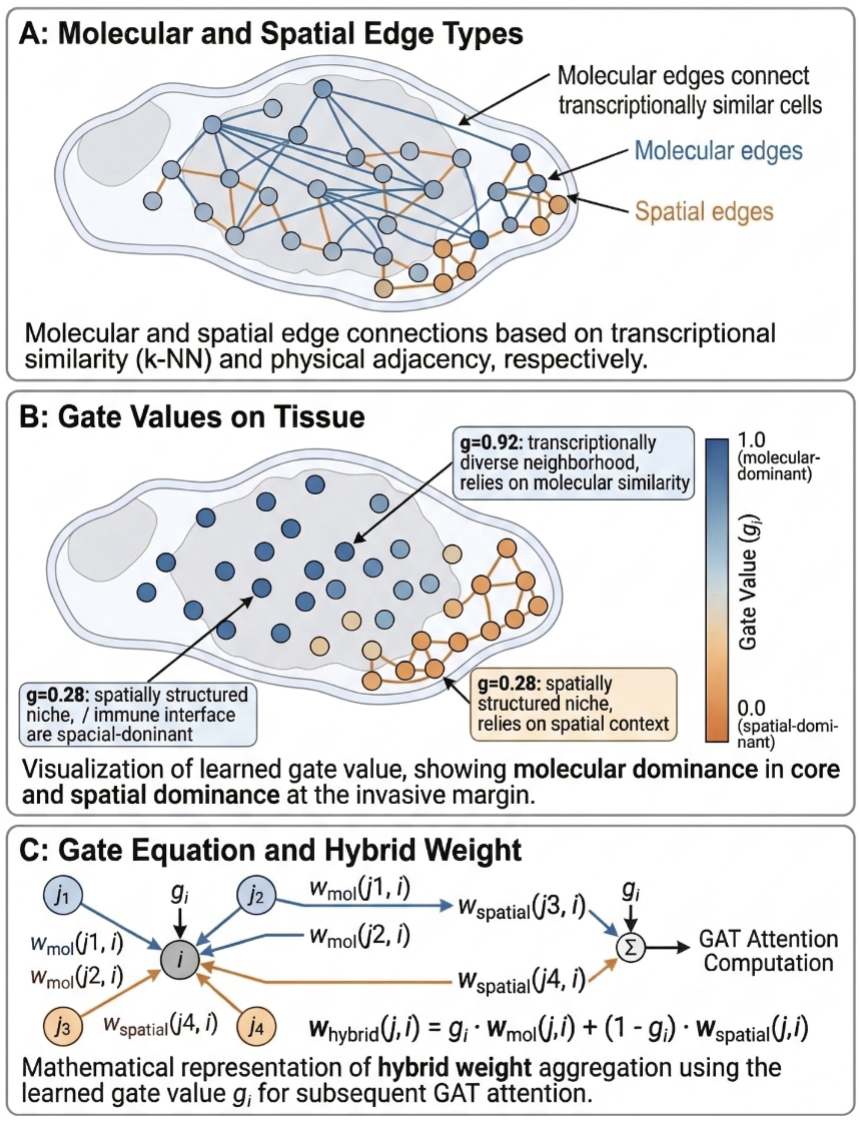
\includegraphics[width=0.75\textwidth]{figuresGVAE/ThreePanelGate.png}
\caption{\textbf{Cell-adaptive gate mechanism for hybrid graph fusion.} \textbf{(A)}~Molecular edges (blue) connect transcriptionally similar cells via $k$-NN in PCA space, while spatial edges (orange) connect physically adjacent cells. \textbf{(B)}~Learned gate values $g_i$ projected onto tissue coordinates reveal spatial structure: cells in the tumor core rely on molecular similarity ($g \approx 0.92$), while cells at the invasive margin and immune interface rely on spatial context ($g \approx 0.28$). \textbf{(C)}~For each target cell $i$, the gate value $g_i$ weights molecular and spatial edge contributions via $w_{\text{hybrid}}(j,i) = g_i \cdot w_{\text{mol}}(j,i) + (1 - g_i) \cdot w_{\text{spatial}}(j,i)$, producing hybrid weights for subsequent GAT attention computation.}
\label{fig:gate}
\end{figure}

\subsubsection{Contrastive Pair Mining}
\label{sec:contrastive_mining}

We mine positive and negative pairs from the graph structure to define a contrastive learning objective (Section~\ref{sec:contrastive}). Positive pairs consist of all spatially adjacent cell pairs (edges in the spatial graph). Negative pairs are constructed by identifying, for each cell, molecular neighbors (cells in its $k$-NN) that are spatially distant (Euclidean distance exceeding $r_{\text{far}} = 5r$, where $r$ is the spatial radius). Up to $k_{\text{neg}} = 10$ negative pairs are sampled per cell. If no spatially distant molecular neighbors exist for a given cell, an adaptive fallback uses the 75th percentile of that cell's $k$-NN Euclidean distances in PCA space as the minimum separation threshold. This mining strategy exploits the biological insight that molecularly similar cells occupying distant spatial niches may represent functionally distinct populations.

\subsubsection{Node Feature Construction}

Node features $\mathbf{X} \in \mathbb{R}^{N \times d}$ are the PCA projections of the log-normalized HVG expression matrix, with $d = 50$ principal components.

\subsection{Graph Variational Autoencoder Architecture}

Our graph variational autoencoder learns a low-dimensional latent representation of cells that captures both their transcriptional state and their position within the cellular interaction network. The architecture consists of an edge-weight-aware graph attention encoder, a zero-inflated negative binomial expression decoder, and an adjacency decoder with negative sampling.

\subsubsection{Encoder Network}

The encoder employs a custom \emph{WeightedGATConv} layer that extends graph attention networks \citep{velickovic2017graph} to incorporate edge weights in the message-passing computation. Standard GAT computes attention-weighted aggregation of neighbor features; our extension additionally multiplies each message by the hybrid edge weight, enabling the model to differentially weight edges based on the cell-adaptive gate output.

For a single attention head $k$ with learnable linear transformation $\mathbf{W}_k$ and attention vector $\mathbf{a}_k$, the attention coefficient for edge $(j, i)$ is:
\begin{equation}
\alpha_{ij}^k = \frac{\exp\left(\text{LeakyReLU}\left(\mathbf{a}_k^T [\mathbf{W}_k \mathbf{x}_i \| \mathbf{W}_k \mathbf{x}_j]\right)\right)}{\sum_{\ell \in \mathcal{N}(i)} \exp\left(\text{LeakyReLU}\left(\mathbf{a}_k^T [\mathbf{W}_k \mathbf{x}_i \| \mathbf{W}_k \mathbf{x}_\ell]\right)\right)}
\end{equation}
where $\|$ denotes concatenation and the LeakyReLU uses a negative slope of 0.2. The message from node $j$ to node $i$ is then:
\begin{equation}
\mathbf{m}_{j \to i}^k = \alpha_{ij}^k \cdot w_{\text{hybrid}}(j, i) \cdot \mathbf{W}_k \mathbf{x}_j
\end{equation}

The encoder consists of two WeightedGATConv layers. The first layer uses $h = 4$ attention heads with concatenation, producing a hidden representation of dimension $H = 64$:
\begin{equation}
\mathbf{H}^{(1)} = \text{ELU}\left(\|_{k=1}^{h} \sum_{j \in \mathcal{N}(i)} \mathbf{m}_{j \to i}^k \right)
\end{equation}
followed by dropout ($p = 0.2$). The second layer produces the variational parameters through two single-head WeightedGATConv layers with mean aggregation:
\begin{align}
\boldsymbol{\mu} &= \text{WeightedGATConv}(\mathbf{H}^{(1)}, \mathbf{A}; \mathbf{W}_{\mu}) \\
\log \boldsymbol{\sigma}^2 &= \text{WeightedGATConv}(\mathbf{H}^{(1)}, \mathbf{A}; \mathbf{W}_{\sigma})
\end{align}

Latent vectors are obtained via the reparameterization trick \citep{kingma2013auto}:
\begin{equation}
\mathbf{z}_i = \boldsymbol{\mu}_i + \exp(0.5 \cdot \log\boldsymbol{\sigma}_i^2) \odot \boldsymbol{\epsilon}, \quad \boldsymbol{\epsilon} \sim \mathcal{N}(\mathbf{0}, \mathbf{I})
\end{equation}

The default latent dimension is $D = 32$.

\subsubsection{Adjacency Decoder with Negative Sampling}

Rather than reconstructing the full $N \times N$ adjacency matrix (computationally prohibitive for large graphs), we employ a negative sampling strategy. For each observed edge $(i, j)$ in the graph, we sample $n_{\text{neg}} = 5$ random non-edges and compute:
\begin{align}
\text{pos\_score}(i,j) &= \sigma(\mathbf{z}_i^T \mathbf{z}_j) \\
\text{neg\_score}(i,k) &= \sigma(\mathbf{z}_i^T \mathbf{z}_k), \quad k \sim \text{Uniform}(1, N)
\end{align}
where $\sigma(\cdot)$ is the sigmoid function. The adjacency reconstruction loss is:
\begin{equation}
\mathcal{L}_{\text{adj}} = -\mathbb{E}_{(i,j) \in \mathcal{E}}[\log \text{pos\_score}(i,j)] - \mathbb{E}_{k \sim \text{neg}}[\log(1 - \text{neg\_score}(i,k))]
\end{equation}

This scales linearly with the number of edges $|\mathcal{E}|$ rather than quadratically with $N$.

\subsubsection{Expression Decoder (ZINB)}

A critical innovation is the inclusion of an expression reconstruction decoder alongside the adjacency decoder. Single-cell RNA-seq count data exhibits zero inflation and overdispersion that are well-modeled by the zero-inflated negative binomial (ZINB) distribution \citep{risso2018general}. The expression decoder maps from the latent representation $\mathbf{z}_i$ back to gene expression space through a multi-layer perceptron backbone with hidden dimensions $[128, 256]$, batch normalization, ELU activations, and dropout ($p = 0.2$) between layers.

Three output heads produce the ZINB parameters for each gene $g$. Let $s_i = \sum_g x_{ig}$ denote the total UMI count (library size) for cell $i$:
\begin{align}
\boldsymbol{\rho}_i &= s_i \cdot \text{softmax}(\mathbf{W}_\rho \mathbf{h}_i) \quad &\text{(rate, scaled by } s_i\text{)} \\
\boldsymbol{\theta} &= \exp(\boldsymbol{\ell}_\theta) \quad &\text{(gene-specific dispersion, shared across cells)} \\
\boldsymbol{\pi}_i &= \sigma(\mathbf{W}_\pi \mathbf{h}_i) \quad &\text{(zero-inflation probability)}
\end{align}
where $\boldsymbol{\ell}_\theta \in \mathbb{R}^G$ is a learnable per-gene log-dispersion parameter.

The ZINB log-likelihood for observed count $x$ given parameters $(\rho, \theta, \pi)$ distinguishes zero and non-zero observations:
\begin{align}
\log p(x = 0) &= \log\left[\pi + (1 - \pi) \left(\frac{\theta}{\theta + \rho}\right)^\theta\right] \\
\log p(x > 0) &= \log(1 - \pi) + \log \Gamma(x + \theta) - \log \Gamma(\theta) - \log \Gamma(x + 1) \nonumber \\
&\quad + \theta \log\frac{\theta}{\theta + \rho} + x \log\frac{\rho}{\theta + \rho}
\end{align}

The expression reconstruction loss is $\mathcal{L}_{\text{expr}} = -\frac{1}{NG}\sum_{i,g} \log p(x_{ig})$.

\subsubsection{Loss Function}

The total training objective combines five loss terms:
\begin{equation}
\label{eq:total_loss}
\mathcal{L} = \mathcal{L}_{\text{adj}} + \lambda_1 \mathcal{L}_{\text{expr}} + \lambda_2 \mathcal{L}_{\text{contrast}} + \beta(t) \mathcal{L}_{\text{KL}} + \gamma \mathcal{L}_{\text{pred}}
\end{equation}

The KL divergence regularizer encourages the latent distribution to remain close to a standard normal prior:
\begin{equation}
\mathcal{L}_{\text{KL}} = -\frac{1}{2N} \sum_{i=1}^N \sum_{d=1}^D \left[ 1 + \log(\sigma_{id}^2) - \mu_{id}^2 - \sigma_{id}^2 \right]
\end{equation}

\paragraph{Contrastive loss.}
\label{sec:contrastive}
The contrastive loss encourages embeddings of spatially proximal cells to be closer than embeddings of molecularly similar but spatially distant cells. We employ an InfoNCE-style objective \citep{oord2018representation} with temperature scaling. Given $L_2$-normalized embeddings $\tilde{\mathbf{z}} = \mathbf{z} / \|\mathbf{z}\|_2$ and mined positive pair $(i, j^+)$ with grouped negatives $\{k_1, \ldots, k_m\}$ sharing anchor $i$:
\begin{equation}
\mathcal{L}_{\text{contrast}} = -\mathbb{E}\left[\log \frac{\exp(\tilde{\mathbf{z}}_i^T \tilde{\mathbf{z}}_{j^+} / \tau)}{\exp(\tilde{\mathbf{z}}_i^T \tilde{\mathbf{z}}_{j^+} / \tau) + \sum_{k} \exp(\tilde{\mathbf{z}}_i^T \tilde{\mathbf{z}}_k / \tau)}\right]
\end{equation}
where $\tau = 0.1$ is the temperature parameter. The log-sum-exp computation uses the max-subtraction trick for numerical stability.

\paragraph{Prediction loss.} The prediction loss $\mathcal{L}_{\text{pred}}$ (detailed in Section~\ref{sec:predictor}) is binary cross-entropy for patient-level immunotherapy response, active only during Phase 2 training ($\gamma > 0$).

\paragraph{Posterior collapse prevention.} Graph convolutional encoders are particularly susceptible to posterior collapse, wherein the powerful message-passing mechanism produces accurate reconstructions while the latent bottleneck carries negligible information ($\text{KL} \to 0$), rendering the VAE's uncertainty estimates meaningless. We employ two complementary mitigations. First, \textit{cyclical KL annealing} \citep{fu2019cyclical}: rather than a single linear warm-up, the KL weight $\beta$ cycles $n_c = 4$ times over Phase~1 training:
\begin{equation}
\beta(t) = \begin{cases}
\beta_{\text{target}} \cdot \frac{t \bmod L}{L/2} & \text{if } (t \bmod L) < L/2 \\
\beta_{\text{target}} & \text{otherwise}
\end{cases}
\end{equation}
where $L = T_{\text{Phase1}} / n_c$ is the cycle length. Each cycle forces the encoder to re-learn an informative latent representation under increasing regularization pressure, preventing early convergence to a degenerate KL-free solution. Second, \textit{free bits} \citep{kingma2016improved}: the per-dimension KL divergence is clamped to a minimum of $\lambda_{\text{fb}} = 0.5$ nats before summation:
\begin{equation}
\mathcal{L}_{\text{KL}}^{\text{fb}} = \frac{1}{N} \sum_{i=1}^N \sum_{d=1}^D \max\left(\text{KL}_{id},\; \lambda_{\text{fb}}\right)
\end{equation}
where $\text{KL}_{id} = \frac{1}{2}(\mu_{id}^2 + \sigma_{id}^2 - \log\sigma_{id}^2 - 1)$. This guarantees that each latent dimension encodes at least $\lambda_{\text{fb}}$ nats of information even when $\beta$ is low, preventing selective posterior collapse where a subset of latent dimensions become inactive.

Default loss weights are $\lambda_1 = 1.0$, $\lambda_2 = 0.5$, $\beta_{\text{target}} = 0.01$, and $\gamma = 0.1$.

\subsection{Two-Phase Training Protocol}

Training proceeds in two phases with distinct objectives (Figure~\ref{fig:training}), optimized using Adam \citep{kingma2014adam} with cosine annealing learning rate scheduling.

\paragraph{Phase 1: Representation Learning.} The prediction loss is disabled ($\gamma = 0$). The model learns to reconstruct graph topology, reconstruct gene expression, and structure the latent space through the KL and contrastive losses. Training uses learning rate $\eta = 10^{-3}$ for up to 300 epochs with early stopping (patience of 50 epochs, evaluated every 10 epochs on validation loss $\mathcal{L}_{\text{adj}} + \mathcal{L}_{\text{expr}}$). The best model state is restored after early stopping. Gradient clipping at max norm 1.0 stabilizes training throughout. Model checkpoints are saved every 50 epochs to enable recovery from interruptions; for NSCLC datasets (200,000+ cells), training budgets are extended to 500 and 300 epochs for Phase 1 and Phase 2 respectively.

\paragraph{Phase 2: Joint Clinical Fine-Tuning.} For datasets with patient-level response annotations, the prediction loss is activated ($\gamma = 0.1$) with a reduced learning rate ($\eta = 10^{-4}$) for up to 200 additional epochs. A reconstruction quality safeguard monitors validation losses: if $\mathcal{L}_{\text{adj}}^{\text{val}} > 1.1 \cdot \mathcal{L}_{\text{adj}}^{\text{Phase1}}$ or $\mathcal{L}_{\text{expr}}^{\text{val}} > 1.1 \cdot \mathcal{L}_{\text{expr}}^{\text{Phase1}}$, the prediction weight $\gamma$ is halved. After three such reductions ($\gamma_{\min} = 0.1/2^3 = 0.0125$), Phase 2 terminates early to preserve representation quality. Optionally, the encoder and gate parameters can be frozen during Phase 2 (training only the predictor head), which serves as an ablation condition.

\paragraph{Mini-batch training.} For datasets exceeding 50,000 cells, we automatically employ mini-batch training using PyTorch Geometric's NeighborLoader with 2-hop neighbor sampling ($[15, 10]$ neighbors per hop) and batch size $B = 512$. This enables processing of arbitrarily large graphs with per-iteration complexity $O(B \cdot k^2 \cdot D \cdot H)$.

\begin{figure}[t]
\centering
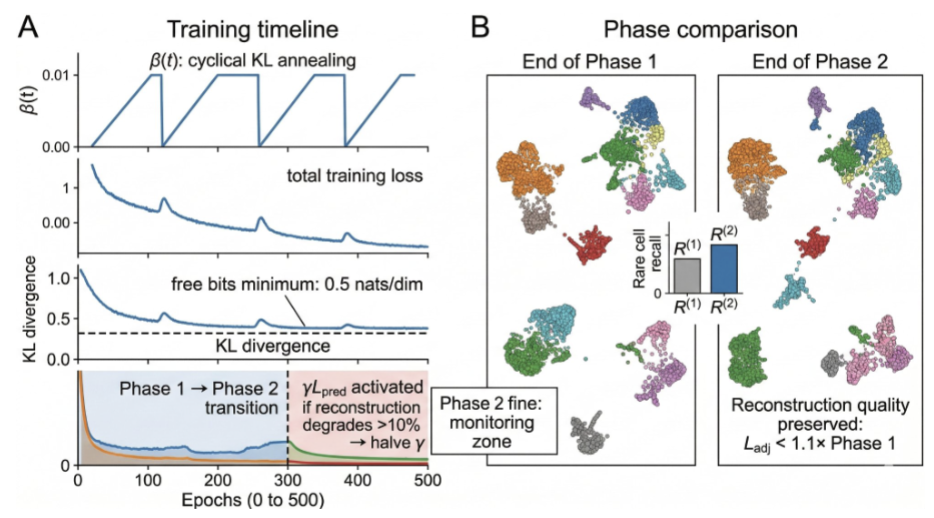
\includegraphics[width=\textwidth]{figuresGVAE/TwoPhasePanels.png}
\caption{\textbf{Two-phase training protocol with posterior collapse prevention.} \textbf{(A)}~Training timeline showing the cyclical KL annealing schedule $\beta(t)$ with 4 ramp-hold cycles, total training loss, and KL divergence maintained above the free bits minimum (0.5 nats/dim, dashed line). The Phase~1 to Phase~2 transition at epoch 300 activates the prediction loss $\gamma \mathcal{L}_{\text{pred}}$; a monitoring zone ensures reconstruction quality remains within 10\% of Phase~1 levels. \textbf{(B)}~Phase comparison of latent space structure: UMAP visualizations at the end of Phase~1 (representation learning only) and Phase~2 (joint clinical fine-tuning) demonstrate that cluster structure and rare cell recall ($R^{(1)}$ vs.\ $R^{(2)}$) are preserved or improved by clinical supervision.}
\label{fig:training}
\end{figure}

\subsection{End-to-End Response Predictor}
\label{sec:predictor}

For patient-level immunotherapy response prediction, we develop an end-to-end predictor that operates directly on cell-level embeddings rather than requiring manual feature engineering.

\paragraph{Attention pooling.} Each patient's cells are aggregated into a single patient-level representation via attention pooling:
\begin{align}
a_i &= \mathbf{v}^T \tanh(\mathbf{W}_a \mathbf{z}_i), \quad i \in \text{cells}(p) \\
\alpha_i &= \frac{\exp(a_i)}{\sum_{j \in \text{cells}(p)} \exp(a_j)} \\
\mathbf{h}_p &= \sum_{i \in \text{cells}(p)} \alpha_i \mathbf{z}_i
\end{align}
where $\mathbf{W}_a \in \mathbb{R}^{D \times D}$ and $\mathbf{v} \in \mathbb{R}^D$ are learnable parameters. The attention weights $\alpha_i$ are interpretable: cells with high attention contribute disproportionately to the prediction, revealing which subpopulations drive response classification.

\paragraph{Classifier.} The patient embedding $\mathbf{h}_p$ is passed through a linear classifier with sigmoid activation:
\begin{equation}
\hat{y}_p = \sigma(\mathbf{w}_c^T \mathbf{h}_p + b_c)
\end{equation}

The prediction loss is binary cross-entropy computed over training patients:
\begin{equation}
\mathcal{L}_{\text{pred}} = -\frac{1}{|\mathcal{P}_{\text{train}}|} \sum_{p \in \mathcal{P}_{\text{train}}} \left[ y_p \log \hat{y}_p + (1 - y_p) \log(1 - \hat{y}_p) \right]
\end{equation}

Patient-level data splits ensure all cells from a given patient are in the same fold (70\% train, 15\% validation, 15\% test by patient).

\subsection{Downstream Analysis and Biological Interpretation}

\subsubsection{KL Divergence-Based Rare Cell Detection}

A key advantage of the variational framework is the ability to identify rare cells through posterior uncertainty. For each cell $i$, the KL divergence from the standard normal prior quantifies how far the cell's latent distribution deviates from the population:
\begin{equation}
\text{KL}_i = \frac{1}{2} \sum_{d=1}^D \left[\mu_{id}^2 + \exp(\log\sigma_{id}^2) - \log\sigma_{id}^2 - 1\right]
\end{equation}

Cells with high KL divergence occupy unusual regions of latent space. We compute z-scores of per-cell KL values and classify cells as rare when $z_{\text{KL}} > \eta$, where $\eta = 2.0$ (two standard deviations above the mean) by default. Rare cells are further subclustered using Leiden community detection at high resolution ($\gamma = 2.0$) with $k = 15$ neighbors in latent space, enabling identification of distinct rare subpopulations. Subcluster labels start at index 100 to distinguish them from main cluster assignments.

\subsubsection{Immunosuppressive Signature Validation}
\label{sec:signature_validation}

To validate that rare cells identified by KL-based detection represent biologically coherent immunosuppressive populations rather than technical artifacts, we score all cells against four curated immunosuppressive gene signatures: regulatory T cells (FOXP3, IL2RA, CTLA4, IKZF2, TNFRSF18), M2-polarized macrophages (CD163, MRC1, MSR1, MARCO, CD209), myeloid-derived suppressor cells (S100A8, S100A9, S100A12, FCN1, VCAN), and exhausted T cells (PDCD1, LAG3, HAVCR2, TIGIT, TOX).

For each signature, the per-cell score is computed as the mean normalized expression of available signature genes. We then compare the distribution of signature scores between rare cells ($z_{\text{KL}} > \eta$) and non-rare cells using the Mann-Whitney U test (two-sided). Effect sizes are quantified as the standardized mean difference (rare mean minus non-rare mean, divided by the pooled standard deviation). A significant enrichment of immunosuppressive signatures among rare cells (after Benjamini-Hochberg FDR correction) provides direct biological evidence that the GVAE's uncertainty-based detection identifies functionally relevant subpopulations.

\subsubsection{Controlled Spike-In Validation}

To provide ground-truth validation of rare cell recovery with realistic expression profiles, we perform a controlled spike-in experiment on the melanoma dataset. We inject known rare populations by selecting a random subset of cells (at controlled fractions of 1\%, 2\%, and 5\% of total cells) and upregulating canonical regulatory T cell markers (FOXP3, IL2RA, CTLA4, IKZF2, TNFRSF18) or MDSC markers (S100A8, S100A9, CD14, ITGAM, ARG1) by a controlled effect size ($e^{1.0}$ or $e^{2.0}$-fold increase in raw counts), followed by renormalization and PCA recomputation. The ground-truth identity of spiked cells is retained for evaluation. We then run the full GVAE pipeline including KL-divergence-based rare cell detection and measure precision, recall, and F1-score of recovering the spiked-in population. This experiment is repeated for each combination of spike-in fraction and effect size across three methods: GVAE (KL-divergence detection), scVI (posterior variance thresholding), and Scanpy (Leiden clustering with frequency-based rare detection), providing a head-to-head comparison of rare cell sensitivity under controlled conditions with known ground truth.

\subsubsection{Rare Subcluster Marker Genes and Pathway Enrichment}

Beyond signature scoring, we perform de novo marker gene discovery specifically on rare subclusters to characterize their transcriptional programs. Differential expression analysis compares each rare subcluster (labels $\geq$ 100) against all other rare subclusters using the Wilcoxon rank-sum test, retaining genes with $|\log_2 \text{FC}| > 1$ and FDR $< 0.01$. Gene Set Enrichment Analysis (GSEA) is then performed on these rare subcluster markers against three complementary gene set libraries: MSigDB Hallmark 2020, GO Biological Process 2023, and KEGG 2021 Human, returning the top 10 enriched terms per subcluster per library. This multi-library approach identifies whether rare subclusters exhibit enrichment for immune evasion, metabolic reprogramming, or signaling pathways associated with immunosuppression.

\subsubsection{Uncertainty-Aware Clustering}

The learned latent representations serve as input for Leiden clustering \citep{traag2019louvain} with automatic resolution selection. We search over $\gamma \in \{0.5, 1.0, 1.5, 2.0\}$ and select the resolution maximizing silhouette score (computed on a subsample of up to 5,000 cells for efficiency). To exploit the probabilistic nature of the latent space, we perform \emph{uncertainty-aware soft assignment}: cell confidence is computed as $\exp(-\overline{\sigma_i^2})$ where $\overline{\sigma_i^2}$ is the mean posterior variance. Cells below the 20th confidence percentile receive soft cluster assignments based on distance to cluster centroids (computed using only high-confidence cells), normalized by the cell's posterior variance:
\begin{equation}
p(c | \mathbf{z}_i) \propto \exp\left(-\frac{\|\mathbf{z}_i - \boldsymbol{\mu}_c\|^2}{2\overline{\sigma_i^2} + \epsilon}\right)
\end{equation}

Cluster stability is assessed via the Adjusted Rand Index (ARI) computed across 20 independent Leiden runs with different random seeds. Mean pairwise ARI above 0.8 indicates robust clustering.

\subsubsection{Marker Gene Discovery and Pathway Enrichment}

Differential expression analysis compares each cluster to all other cells using the Wilcoxon rank-sum test with Benjamini-Hochberg FDR correction, retaining genes with $|\log_2 \text{FC}| > 1$ and FDR $< 0.01$ (falling back to the top 50 genes by rank if fewer than 5 pass the filter). Gene Set Enrichment Analysis (GSEA) \citep{subramanian2005gene} is performed on marker gene sets against MSigDB Hallmark 2020 pathways using the Enrichr interface, returning the top 10 enriched terms per cluster.

\subsubsection{Cell Type Annotation}

Cell type annotation uses CellTypist \citep{dominguez2022cross} with the Immune\_All\_Low reference model and majority voting across local neighborhoods. For datasets with matched scRNA-seq references, a dataset-specific CellTypist model is trained on the reference with stochastic gradient descent and applied to the target data.

\subsubsection{Ligand-Receptor Interaction Scoring}

We score ligand-receptor interactions across cell type pairs using a curated set of 24 immune-relevant L-R pairs spanning chemokines (CCL5--CCR5, CXCL9--CXCR3, CXCL13--CXCR5, CCL19--CCR7, CCL21--CCR7), immune checkpoints (CD274--PDCD1, CD80--CD28, CD86--CTLA4, LGALS9--HAVCR2), co-stimulatory molecules (TNFSF9--TNFRSF9), death receptors (FAS--FASLG), cytokines (IFNG--IFNGR1, TNF--TNFRSF1A, IL2--IL2RA, IL10--IL10RA, TGFB1--TGFBR1), MHC--KIR interactions (HLA-A--KIR2DL1, HLA-B--KIR3DL1), angiogenic factors (VEGFA--FLT1, VEGFA--KDR), and adhesion molecules (SPP1--CD44). The interaction score for L-R pair $(l, r)$ between source cluster $s$ and target cluster $t$ is:
\begin{equation}
\text{score}(l, r, s, t) = \bar{x}_{l,s} \cdot \bar{x}_{r,t}
\end{equation}
where $\bar{x}_{l,s}$ is the mean expression of ligand $l$ in cluster $s$. Results are exported in CellPhoneDB-compatible format for downstream analysis.

\subsubsection{Attention Weight Analysis}

The learned attention weights from the WeightedGATConv encoder provide interpretable information about which cellular interactions the model has identified as important. For multi-head attention, weights are averaged across heads. For each target node $i$ with neighbor set $\mathcal{N}(i)$, let $\hat{\alpha}_{ij}$ denote the normalized attention weight (summing to one over neighbors). We compute the attention \emph{selectivity} as the KL divergence from the uniform distribution $\mathcal{U}_{|\mathcal{N}(i)|}$:
\begin{equation}
S_i = D_{\text{KL}}\!\left(\hat{\boldsymbol{\alpha}}_i \,\|\, \mathcal{U}_{|\mathcal{N}(i)|}\right) = \sum_{j \in \mathcal{N}(i)} \hat{\alpha}_{ij} \log \left(|\mathcal{N}(i)| \cdot \hat{\alpha}_{ij}\right)
\end{equation}
High selectivity ($S_i \gg 0$) indicates that the cell preferentially attends to specific neighbors rather than aggregating uniformly. Aggregating high-selectivity edges (above the 75th percentile) by cell type produces a cell type interaction network revealing dominant communication axes within the TME.

\paragraph{Novel interaction discovery.} A key limitation of validation against known ligand-receptor databases is that it can only confirm established biology, not reveal new signaling mechanisms. To address this, we partition all high-attention edges (above the 90th percentile of mean attention across heads) into two categories: \textit{L-R matched} edges where source and target cells co-express at least one known ligand-receptor pair from the curated set of 24 immune-relevant pairs, and \textit{novel} edges with no detectable ligand-receptor co-expression. For novel high-attention edges, we characterize the underlying biology by computing differentially expressed genes between source and target cell populations (Wilcoxon rank-sum, FDR $< 0.05$, $|\log_2\text{FC}| > 1$) and performing Gene Ontology enrichment analysis on the resulting gene signatures. This analysis directly addresses whether the attention mechanism captures interactions beyond curated databases, with the fraction of novel edges and their associated gene programs providing candidate hypotheses for previously uncharacterized cell-cell communication in the TME.

\subsubsection{Spatial Validation}
\label{sec:spatial_validation}

For spatial transcriptomics datasets, we validate the biological coherence of the learned gate values through Moran's I statistic, which quantifies spatial autocorrelation. Given gate values $g_i$ and spatial coordinates, the statistic is computed with $k = 15$ nearest spatial neighbors:
\begin{equation}
I = \frac{N}{W} \frac{\sum_{i} \sum_{j} w_{ij}(g_i - \bar{g})(g_j - \bar{g})}{\sum_{i}(g_i - \bar{g})^2}
\end{equation}
where $W = \sum_{i,j} w_{ij}$. Significance is assessed via a z-test under the normality assumption, and confirmed by a permutation test with 1,000 iterations comparing the observed $I$ to a null distribution generated by random shuffling of gate values.

\subsubsection{Batch Mixing Assessment}
\label{sec:batch_mixing}

To evaluate whether latent representations exhibit batch effects, we compute two complementary metrics. The k-nearest neighbor Batch Effect Test (kBET) \citep{buttner2019test} tests whether the batch label distribution in each cell's local neighborhood ($k = 50$) deviates from the global distribution via chi-squared tests (subsampling to 5,000 cells for computational efficiency). The rejection rate (fraction of cells with significant local deviation at $\alpha = 0.05$) quantifies batch mixing quality, where lower is better. We additionally compute the mean normalized Shannon entropy of batch labels in $k$-NN neighborhoods:
\begin{equation}
\bar{H} = \frac{1}{N} \sum_{i=1}^N \frac{-\sum_b p_{b,i} \log p_{b,i}}{\log B}
\end{equation}
where $p_{b,i}$ is the proportion of batch $b$ in cell $i$'s neighborhood and $B$ is the total number of batches. Values near 1.0 indicate ideal mixing.

\subsubsection{Clinical Association Testing}

For rare cell subpopulations identified by KL-based detection, we test their association with immunotherapy response via logistic regression:
\begin{equation}
\text{logit}(P(\text{response})) = \beta_0 + \sum_{c} \beta_c f_{p,c} + \sum_{t} \beta_t \mathbb{I}[\text{therapy}_p = t]
\end{equation}
where $f_{p,c}$ is the fraction of patient $p$'s cells belonging to rare subcluster $c$, and therapy type is included as a covariate when available. The model is fit using maximum likelihood estimation (statsmodels Logit, maxiter = 500). Statistical significance is assessed via Wald tests with Benjamini-Hochberg FDR correction for multiple comparisons across rare subclusters.

\subsection{Baseline Comparison}
\label{sec:baselines}

To contextualize the performance of our GVAE framework, we benchmark against two established methods that represent the current standard of practice: a deep generative model (scVI) and a conventional clustering workflow (Scanpy standard pipeline). All methods are evaluated on identical data (same HVG-filtered AnnData objects) with shared patient-level cross-validation splits to ensure fair comparison.

\subsubsection{scVI Baseline}

scVI (single-cell Variational Inference) \citep{lopez2018deep} serves as the deep learning baseline, representing the state of the art in VAE-based single-cell analysis. Unlike our GVAE, scVI does not model cell-cell relationships or integrate spatial information. We train scVI with the same latent dimension ($D = 32$) and up to 200 epochs with early stopping, using the raw count layer when available. Latent embeddings are extracted and subjected to the same downstream analyses: Leiden clustering with silhouette-based resolution selection, and L1-regularized logistic regression on per-patient features (mean embedding, cluster proportions, Shannon diversity) for response prediction. For rare cell detection, we estimate per-cell uncertainty by drawing 20 stochastic samples from the posterior and computing per-cell variance; cells with variance z-scores exceeding 2.0 are classified as rare.

\subsubsection{Scanpy Standard Workflow Baseline}

The Scanpy baseline represents the conventional non-deep-learning workflow: PCA (50 components), $k$-NN graph construction ($k = 15$), and Leiden clustering at resolution 1.0. This pipeline treats cells as independent observations with no learned representation beyond linear PCA. For response prediction, L1-regularized logistic regression is applied to per-patient features extracted from PCA embeddings and cluster proportions (same feature construction as the scVI baseline). Rare cells are identified by frequency thresholding: clusters comprising less than 1\% of the total cell population are classified as rare.

\subsubsection{Benchmark Evaluation}

All three methods (GVAE, scVI, Scanpy) are evaluated using stratified 5-fold cross-validation with identical patient-level splits. We report AUROC and AUPRC for response prediction, silhouette score for clustering quality, and the number of rare cells detected. This head-to-head comparison isolates the contribution of graph-based multi-modal integration (GVAE) beyond what is achievable with a standard VAE (scVI) or conventional workflow (Scanpy).

\subsection{Cross-Dataset Transfer Validation}
\label{sec:transfer}

To assess the generalizability of learned representations beyond the training dataset, we perform cross-dataset transfer experiments. A GVAE model trained on the melanoma cohort (32 patients) is applied to the NSCLC ICI cohort (243 patients) without retraining the encoder or gate parameters.

The transfer procedure operates as follows. First, we identify the intersection of highly variable genes between the source and target datasets (requiring at least 500 shared genes). The target dataset is subset to shared genes and PCA is recomputed to match the source model's input dimensionality. A new cellular graph is constructed for the target data using the same graph construction parameters ($k = 15$ molecular neighbors). The frozen source encoder then produces latent embeddings for all target cells.

Transfer quality is evaluated through: (1) clustering quality on target embeddings (silhouette score), confirming that the learned representations capture meaningful biological structure in an unseen cancer type; (2) rare cell detection on target data using the same KL divergence threshold, testing whether the uncertainty-based detection mechanism generalizes; and (3) Jaccard concordance of rare subcluster marker genes between source and target, quantifying whether the model identifies transcriptionally similar rare populations across cancer types. High marker concordance would indicate that the GVAE learns generalizable signatures of immunosuppressive cell states rather than dataset-specific patterns.

\subsection{Ablation Studies}
\label{sec:ablations}

We perform systematic ablation studies across 13 conditions to quantify the contribution of each architectural component:

\begin{table}[H]
\centering
\caption{Ablation conditions and the model component removed or modified.}
\label{tab:ablations}
\begin{tabular}{ll}
\toprule
Ablation & Modification \\
\midrule
\texttt{mol\_only} & Gate fixed to $g = 1$ (molecular edges only) \\
\texttt{spatial\_only} & Gate fixed to $g = 0$ (spatial edges only) \\
\texttt{static\_0.3/0.5/0.7} & Gate fixed to constant $\alpha \in \{0.3, 0.5, 0.7\}$ \\
\texttt{spatial\_bias} & Gate bias initialized to $b = -1.0$ ($g_i \approx 0.27$) \\
\texttt{no\_expr} & Expression reconstruction disabled ($\lambda_1 = 0$) \\
\texttt{gaussian} & Gaussian NLL decoder replaces ZINB \\
\texttt{no\_contrastive} & Contrastive loss disabled ($\lambda_2 = 0$) \\
\texttt{frozen\_encoder} & Encoder and gate frozen during Phase 2 \\
\texttt{gcn\_encoder} & GCNConv replaces WeightedGATConv (no attention) \\
\texttt{rare\_leiden} & Leiden-only rare cell detection (no KL scores) \\
\texttt{logreg\_baseline} & L1-logistic regression on hand-crafted features \\
\bottomrule
\end{tabular}
\end{table}

The GCN encoder ablation replaces WeightedGATConv with standard GCNConv layers \citep{kipf2016semi}, removing the attention mechanism while preserving the same hidden and latent dimensions. The Gaussian decoder ablation replaces the ZINB likelihood with a Gaussian negative log-likelihood $\mathcal{L}_{\text{expr}} = \frac{1}{2}(\log\sigma^2 + (x - \mu)^2 / (\exp(\sigma^2) + \epsilon))$, with per-gene learnable mean and variance heads. The spatial bias ablation compares the default gate initialization ($b = 0$, yielding $g_i \approx 0.5$) against biased initialization ($b = -1.0$, yielding $g_i \approx 0.27$), evaluating rare cell detection recall for spatially-restricted immunosuppressive populations, spatial niche coherence, and convergence of the learned gate distribution after training.

The logistic regression baseline extracts per-patient features comprising the mean latent vector ($D$ dimensions), cluster proportions ($C$ dimensions), and Shannon diversity (1 dimension), then applies L1-regularized logistic regression (solver: SAGA, $C = 1.0$, max iterations = 5,000) with stratified 5-fold cross-validation. This baseline tests whether the end-to-end attention-pooling predictor provides value beyond simple feature extraction from the learned embeddings.

\subsection{Model Validation and Statistical Rigor}

\subsubsection{Cross-Validation Protocol}

Predictive performance is evaluated via nested cross-validation. The outer loop uses stratified 5-fold patient-level splits for performance evaluation. An optional inner loop performs hyperparameter selection from a grid of 5 configurations varying latent dimension $D \in \{16, 32, 64\}$ and expression loss weight $\lambda_1 \in \{0.5, 1.0, 2.0\}$, each trained with reduced budget (100 epochs, patience 15). The hidden dimension is adjusted to $H = h \cdot \lfloor D / h \rfloor$ to ensure compatibility with the number of attention heads $h$.

We report area under the receiver operating characteristic curve (AUROC), area under the precision-recall curve (AUPRC), balanced accuracy, precision, recall, specificity, and F1 score. Confidence intervals are computed via bootstrap resampling with 1,000 iterations at the 95\% level ($\alpha/2$ and $1-\alpha/2$ percentiles). Statistical significance of predictions is assessed via permutation testing: patient labels are shuffled 1,000 times, and the $p$-value is the fraction of null AUROCs equaling or exceeding the observed AUROC.

\subsubsection{Hyperparameter Optimization}

Hyperparameters are optimized using Bayesian optimization via the Optuna framework \citep{akiba2019optuna} with Tree-structured Parzen Estimator (TPE) sampling. We allocate 50 trials (10 random startup trials followed by 40 guided trials), each training for 100 epochs with patience 20. The validation objective combines reconstruction loss with a biological coherence term:
\begin{equation}
\mathcal{J} = \mathcal{L}_{\text{adj}}^{\text{val}} + \lambda_1 \mathcal{L}_{\text{expr}}^{\text{val}} + \lambda_2 \mathcal{L}_{\text{contrast}}^{\text{val}} + \beta \mathcal{L}_{\text{KL}}^{\text{val}} - 0.1 \cdot S_{\text{sil}}
\end{equation}
where $S_{\text{sil}}$ is the silhouette score of $k$-means clustering on the latent embeddings, included to prevent selection of configurations that minimize reconstruction loss through memorization rather than learning biologically coherent representations.

The search space is:

\begin{table}[H]
\centering
\caption{Hyperparameter search space for Optuna optimization.}
\label{tab:hpsearch}
\begin{tabular}{ll}
\toprule
Parameter & Search Space \\
\midrule
$k_{\text{mol}}$ (molecular neighbors) & $\{10, 15, 20, 30\}$ \\
Latent dimension $D$ & $\{16, 32, 64\}$ \\
Attention heads $h$ & $\{1, 2, 4, 8\}$ \\
$\lambda_1$ (expression weight) & $\{0.1, 0.5, 1.0, 2.0\}$ \\
$\lambda_2$ (contrastive weight) & $\{0.1, 0.5, 1.0\}$ \\
$\beta$ (KL weight) & $\{0.001, 0.01, 0.1\}$ \\
$\gamma$ (prediction weight) & $\{0.01, 0.05, 0.1, 0.5\}$ \\
$\tau$ (temperature) & $\{0.05, 0.1, 0.2, 0.5\}$ \\
$\eta$ (rare threshold) & $\{1.5, 2.0, 2.5, 3.0\}$ \\
$n_{\text{neg}}$ (negative samples) & $\{5, 10, 20\}$ \\
$\lambda_{\text{fb}}$ (free bits) & $\{0, 0.25, 0.5, 1.0\}$ nats \\
\bottomrule
\end{tabular}
\end{table}

After optimization, the top-3 configurations are retrained at full budget (300 epochs), and the best is selected by the combined objective $\mathcal{J}$.

\subsubsection{Reproducibility}

All stochastic procedures use fixed random seeds (random state = 42). Code, trained models, and configuration files are released as open-source software at \url{https://github.com/YCRG-Labs/gvae-tme} with a comprehensive test suite covering model architecture, training, loss functions, ablations, clustering, batch mixing, spatial validation, and configuration integrity. A unified benchmarking script (\texttt{benchmark.py}) enables reproduction of all baseline comparisons and cross-dataset transfer experiments with a single command.

\newpage
\bibliographystyle{plainnat}
\bibliography{referencesfixed}

\appendix
\section{Computational Complexity Analysis}

\paragraph{Graph Construction.}
Exact $k$-NN search requires computing $O(N^2 d)$ distances where $N$ is the number of cells and $d$ is the PCA dimension. Approximate nearest neighbor methods via Annoy reduce this to $O(N \log N \cdot d)$ through random projection trees (50 trees). Spatial graph construction uses $k$-d tree range queries with complexity $O(N \log N)$.

\paragraph{GVAE Training.}
Each forward pass of the WeightedGATConv encoder requires $O(|\mathcal{E}| \cdot D \cdot H)$ operations where $|\mathcal{E}|$ is the number of edges, $D$ is the hidden dimension, and $H$ is the number of attention heads. For sparse $k$-NN graphs with $|\mathcal{E}| = O(N \cdot k)$, this becomes $O(N \cdot k \cdot D \cdot H)$ which scales linearly with the number of cells. The adjacency decoder with negative sampling scales as $O(|\mathcal{E}| \cdot n_{\text{neg}} \cdot D)$ rather than the $O(N^2 D)$ required for full reconstruction. The ZINB decoder scales as $O(N \cdot G)$ where $G$ is the number of genes. Mini-batch training with NeighborLoader reduces per-iteration complexity to $O(B \cdot k^2 \cdot D \cdot H)$ where $B$ is the batch size, with the $k^2$ factor arising from 2-hop neighbor sampling.

\paragraph{Sparse Matrix Operations.}
Graph adjacency matrices are stored in COO format compatible with PyTorch Geometric's message-passing interface. Molecular and spatial edge weights are maintained as separate tensors indexed by the unified edge list, enabling efficient hybrid weight computation through the cell-adaptive gate without materializing dense matrices.

\section{Default Hyperparameters}

Table~\ref{tab:defaults} lists the default hyperparameters used for full-scale training.

\begin{table}[H]
\centering
\caption{Default hyperparameters for the GVAE framework (full configuration).}
\label{tab:defaults}
\begin{tabular}{llr}
\toprule
Category & Parameter & Default Value \\
\midrule
Architecture & Hidden dimension & 64 \\
& Latent dimension & 32 \\
& Attention heads & 4 \\
& Dropout & 0.2 \\
& ZINB decoder hidden dims & [128, 256] \\
& Negative samples & 5 \\
\midrule
Loss weights & $\lambda_1$ (expression) & 1.0 \\
& $\lambda_2$ (contrastive) & 0.5 \\
& $\beta_{\text{target}}$ (KL) & 0.01 \\
& $\gamma$ (prediction, Phase 2) & 0.1 \\
& $\tau$ (temperature) & 0.1 \\
& $\lambda_{\text{fb}}$ (free bits) & 0.5 nats \\
\midrule
Training & Learning rate (Phase 1) & $10^{-3}$ \\
& Learning rate (Phase 2) & $10^{-4}$ \\
& Scheduler & Cosine annealing \\
& Epochs (Phase 1) & 300$^\ddagger$ \\
& Epochs (Phase 2) & 200$^\ddagger$ \\
& Patience & 50 \\
& Gradient clip norm & 1.0 \\
& KL annealing cycles & 4 \\
\midrule
Graph & $k_{\text{mol}}$ (molecular neighbors) & 15 \\
& $r_{\text{spatial}}$ & 82.5$\mu$m (Visium) / 24$\mu$m (HD) \\
& $r_{\text{far}}$ factor & 5.0 \\
& $k_{\text{neg}}$ (contrastive negatives) & 10 \\
\midrule
Analysis & Rare threshold $\eta$ & 2.0 \\
& Leiden resolutions & $\{0.5, 1.0, 1.5, 2.0\}$ \\
& ARI stability runs & 20 \\
& Bootstrap iterations & 1,000 \\
& Permutation iterations & 1,000 \\
\midrule
Mini-batch & Batch size & 512 \\
& Neighbor sampling & [15, 10] \\
& Auto-trigger threshold & 50,000 cells \\
\bottomrule
\multicolumn{3}{l}{\footnotesize $^\ddagger$NSCLC datasets use 500/300 epochs (Phase 1/Phase 2) due to larger cell counts.}
\end{tabular}
\end{table}

\end{document}
